\documentclass[12pt, a4paper]{article}
% --- Packages ---
\usepackage[utf8]{inputenc}
\usepackage[T1]{fontenc}
\usepackage[french]{babel}
\usepackage{graphicx} % Make sure this is here for images
\usepackage{booktabs}
\usepackage{amsmath}
\usepackage{geometry}
\usepackage{array}
\usepackage{enumitem}
\usepackage{hyperref}
\usepackage{xcolor}
\usepackage{titlesec}
\usepackage{lmodern}
\usepackage{microtype}
\usepackage{fancyhdr}
\usepackage{listings} % Added for code/JSON display
\usepackage[scaled=0.85]{beramono} % Added for a nicer monospaced font

% --- Font Configuration ---
% --- Color Definitions ---
\definecolor{primary}{RGB}{0,51,102}
\definecolor{secondary}{RGB}{102,102,153}
\definecolor{accent}{RGB}{204,0,0}
\definecolor{codegray}{rgb}{0.5,0.5,0.5}
\definecolor{codepurple}{rgb}{0.58,0,0.82}
\definecolor{codeblue}{rgb}{0,0,0.9}
\definecolor{codegreen}{rgb}{0.1,0.6,0.1} % Darker green for comments

% --- Page Geometry ---
\geometry{
  a4paper,
  left=2.5cm,
  right=2.5cm,
  top=2.5cm,
  bottom=2.5cm,
  headheight=15pt
}
% --- Header/Footer Setup ---
\pagestyle{fancy}
\fancyhf{}
\fancyhead[L]{\small Rapport de Stage - Semaine 4 - Jour 3} % Updated
\fancyhead[R]{\small Zakaria el Khaldi}
\fancyfoot[C]{\thepage}
\renewcommand{\headrulewidth}{0.4pt}
\renewcommand{\footrulewidth}{0.4pt}
% --- Title Formatting ---
\titleformat{\section}
  {\normalfont\Large\bfseries\color{primary}}
  {\thesection}{1em}{}
\titleformat{\subsection}
  {\normalfont\large\bfseries\color{secondary}}
  {\thesubsection}{1em}{}
\titleformat{\subsubsection}
  {\normalfont\normalsize\bfseries\color{accent}}
  {\thesubsubsection}{1em}{}
% --- List Formatting ---
\setlist[itemize]{leftmargin=*, nosep}
\setlist[enumerate]{leftmargin=*, nosep}
% --- Hyperlink Setup ---
\hypersetup{
  colorlinks=true,
  linkcolor=primary,
  urlcolor=secondary,
  citecolor=accent
}

% --- Listings Setup for JSON ---
\lstdefinestyle{json}{
    language=json,
    basicstyle=\ttfamily\footnotesize,
    numbers=left,
    numberstyle=\tiny\color{codegray},
    stepnumber=1,
    numbersep=5pt,
    backgroundcolor=\color{white!95!black}, % Very light gray background
    showspaces=false,
    showstringspaces=false,
    showtabs=false,
    frame=tb, % Top and bottom frame
    framextopmargin=3pt,
    framexbottommargin=3pt,
    rulecolor=\color{black!30!white},
    tabsize=2,
    captionpos=b,
    breaklines=true,
    breakatwhitespace=false,
    stringstyle=\color{codepurple},
    commentstyle=\color{codegreen},
    keywordstyle=\color{codeblue}, % For true, false, null
    morestring=[b]",
    literate=
     *{0}{{{\color{codeblue}0}}}{1}
      {1}{{{\color{codeblue}1}}}{1}
      {2}{{{\color{codeblue}2}}}{1}
      {3}{{{\color{codeblue}3}}}{1}
      {4}{{{\color{codeblue}4}}}{1}
      {5}{{{\color{codeblue}5}}}{1}
      {6}{{{\color{codeblue}6}}}{1}
      {7}{{{\color{codeblue}7}}}{1}
      {8}{{{\color{codeblue}8}}}{1}
      {9}{{{\color{codeblue}9}}}{1}
      {:}{{{\color{black}:}}}{1}
      {\{}{{{\color{black}{\{}}}}{1}
      {\}}{{{\color{black}{\}}}}}{1}
      {[}{{{\color{black}{[}}}}{1}
}


% --- Title Page Information ---
\title{\Huge\bfseries\color{primary} Rapport de Stage \\ 
      \Large Semaine 4 - Jour 3 : Développement des Interfaces de Pratique Spécialisées} % Updated title
\author{\Large Zakaria el Khaldi}
\date{\large Le 29 mai 2025} % Updated date for Day 3, Week 4 (Wednesday, document dated for next day)

% --- Document Start ---
\begin{document}
% --- Cover Page ---
\begin{titlepage}
  \centering
  \vspace*{\stretch{0.5}}
  {\Huge\bfseries\color{primary} Rapport de Stage \par}
  \vspace{1cm}
  {\Large\itshape Semaine 4 - Jour 3 : Implémentation des Environnements de Pratique Interactive\par} % Updated title
  \vspace{2cm}
  
  \vspace{2cm}
  {\Large Zakaria el Khaldi\par}
  \vfill
  {\large Le 28 mai 2025\par} % Date of activity day
  \vspace*{\stretch{1}}
\end{titlepage}

% --- Table of Contents ---
\tableofcontents
\thispagestyle{empty}
\newpage

% --- Introduction ---
\section{Introduction}
\thispagestyle{fancy}
Ce troisième jour de la quatrième semaine de stage a été dédié à l'implémentation de diverses interfaces de pratique spécialisées au sein de la plateforme LearnExpert Premium. L'objectif était de fournir aux utilisateurs des environnements interactifs et ciblés pour développer leurs compétences dans des domaines techniques clés. Ces interfaces sont conçues pour offrir une expérience d'apprentissage "par la pratique" (hands-on), essentielle pour la maîtrise des concepts. Une attention continue a été portée à l'ergonomie et à la clarté pour garantir une prise en main intuitive.

% --- Day's Accomplishments ---
\section{Activités du Jour (Mercredi 28 Mai 2025)} % Updated day and date

\subsection{Développement des Interfaces de Pratique Spécialisées}
La journée a été productive, avec la mise en place de plusieurs modules de pratique interactifs, chacun visant un domaine de compétence spécifique.

\subsubsection{Interface de Pratique d'Algorithmes et Structures de Données}
Une interface inspirée de plateformes comme LeetCode a été développée pour permettre aux utilisateurs de s'exercer sur des problèmes d'algorithmique et de structures de données. Elle comprend un éditeur de code, la description du problème, des exemples de tests et une console pour visualiser les résultats d'exécution. (Voir Figure \ref{fig:leetcode_practice}).

\begin{figure}[htbp]
  \centering
  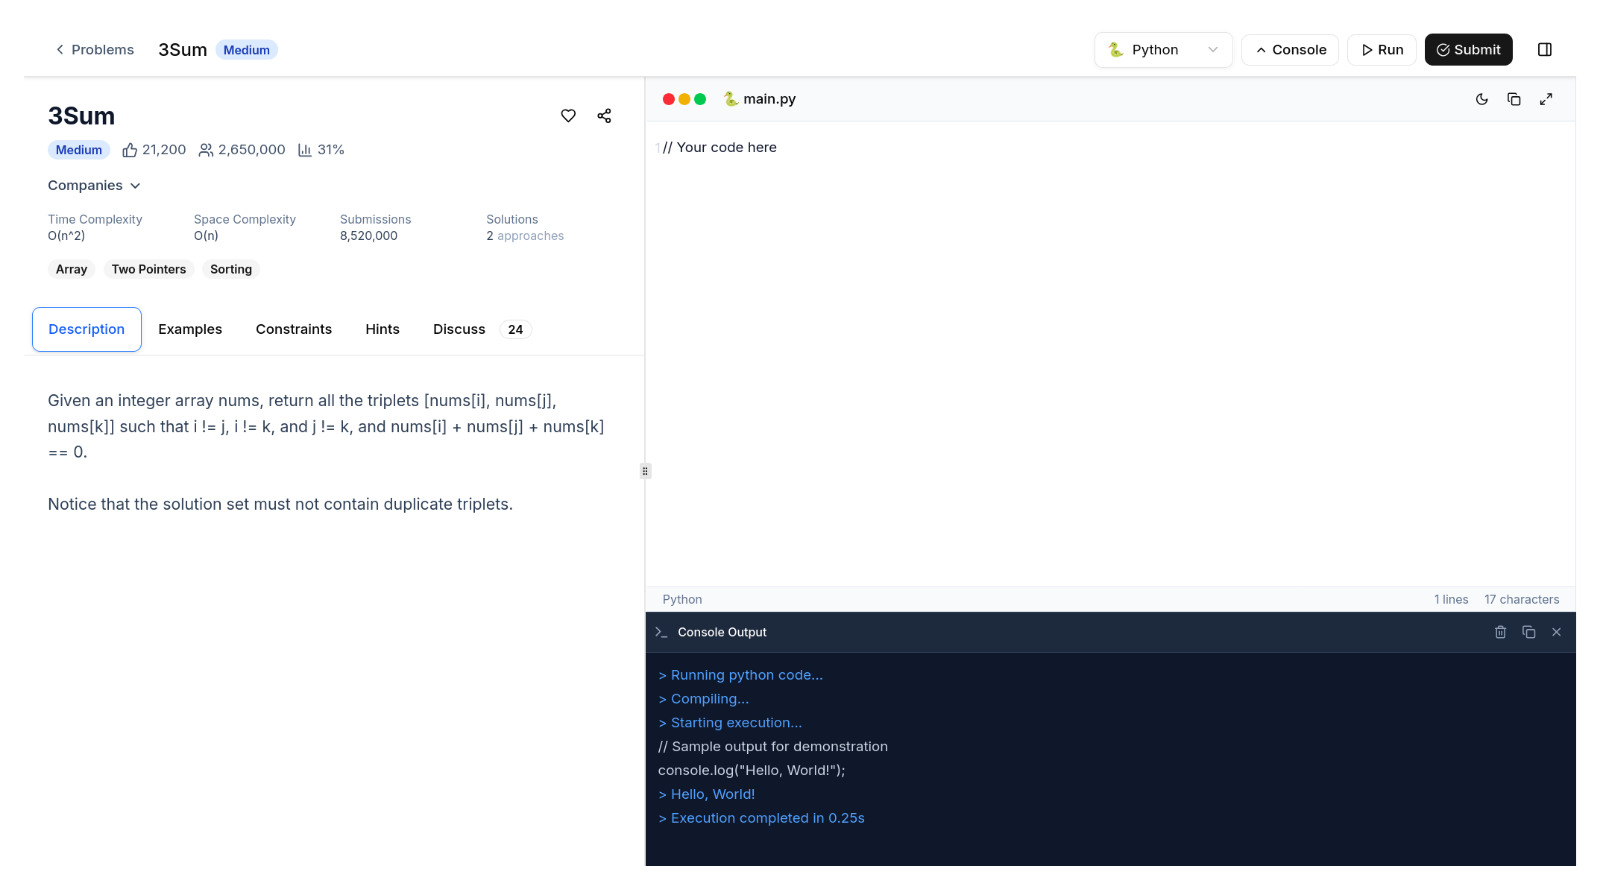
\includegraphics[width=0.85\textwidth]{leetcode.jpeg} % Replace with your leetcode-like image file
  \caption{Interface de pratique pour les algorithmes et structures de données.}
  \label{fig:leetcode_practice}
\end{figure}

\subsubsection{Interface de Pratique en Cybersécurité}
Pour les utilisateurs intéressés par la cybersécurité et le hacking éthique, une interface de type "sandbox" (similaire à TryHackMe) a été implémentée. Elle propose des scénarios de défis et permet d'interagir avec des environnements virtuels pour identifier et exploiter des vulnérabilités de manière contrôlée. (Voir Figure \ref{fig:cybersecurity_practice}).

\begin{figure}[htbp]
  \centering
  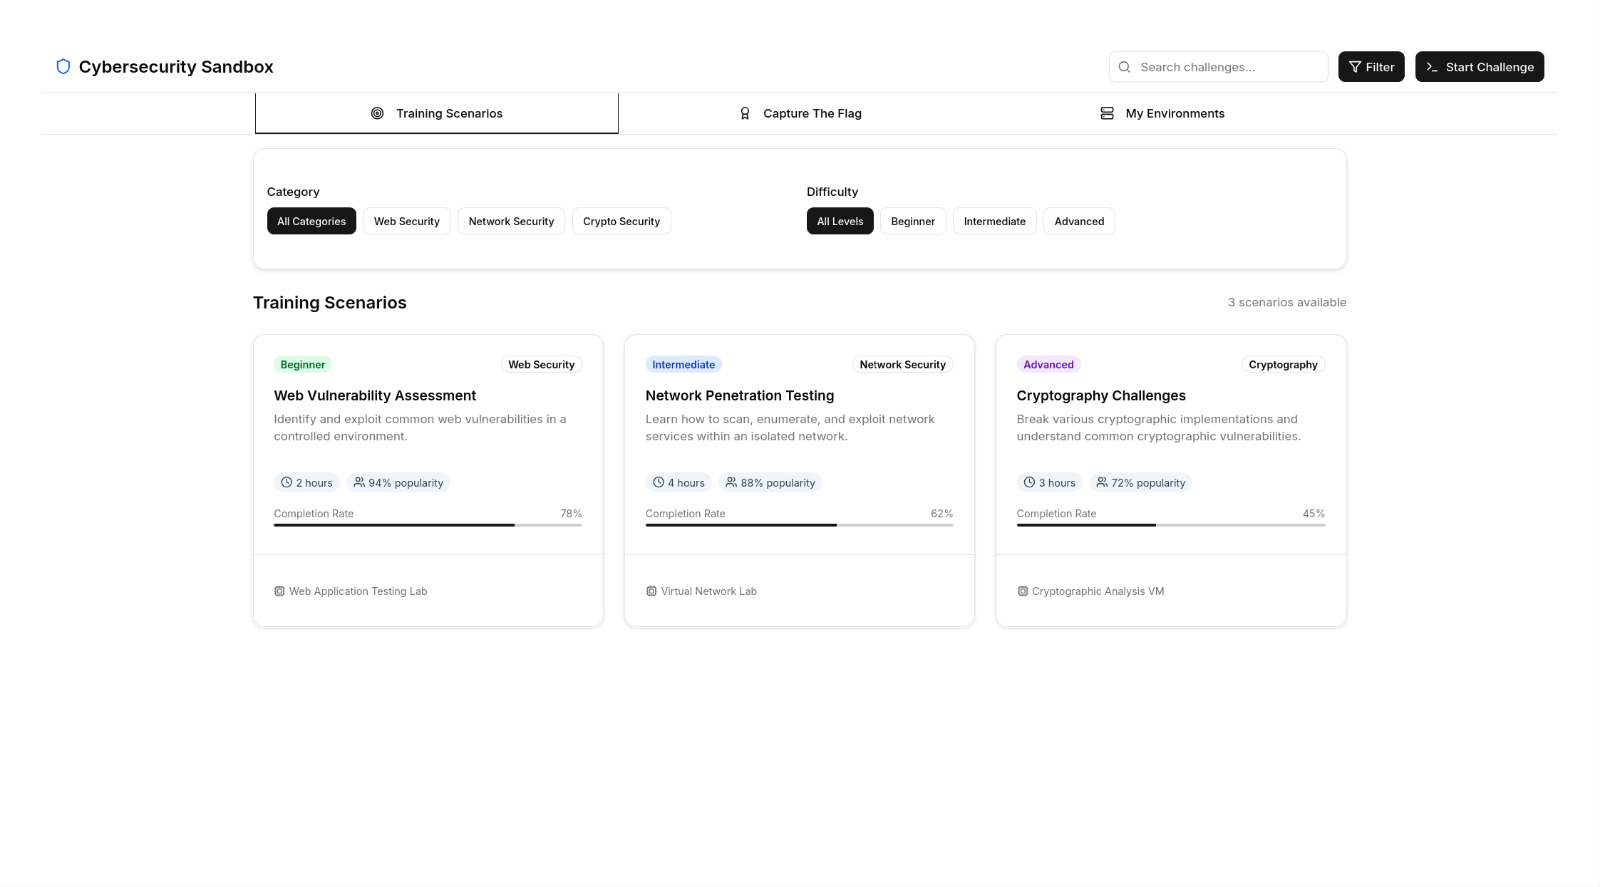
\includegraphics[width=0.85\textwidth]{syber.jpeg} % Replace with your cybersecurity practice image file
  \caption{Environnement de pratique en cybersécurité avec des scénarios de défis.}
  \label{fig:cybersecurity_practice}
\end{figure}

\subsubsection{Interface de Pratique Orientée Systèmes et Réseaux (IT)}
Une page de pratique orientée IT a été mise en place, offrant par exemple un accès terminal à des machines virtuelles préconfigurées. Cela permet aux utilisateurs de s'entraîner à l'administration de serveurs, à la configuration réseau, ou à l'utilisation d'outils en ligne de commande spécifiques. (Voir Figure \ref{fig:it_practice}).

\begin{figure}[htbp]
  \centering
  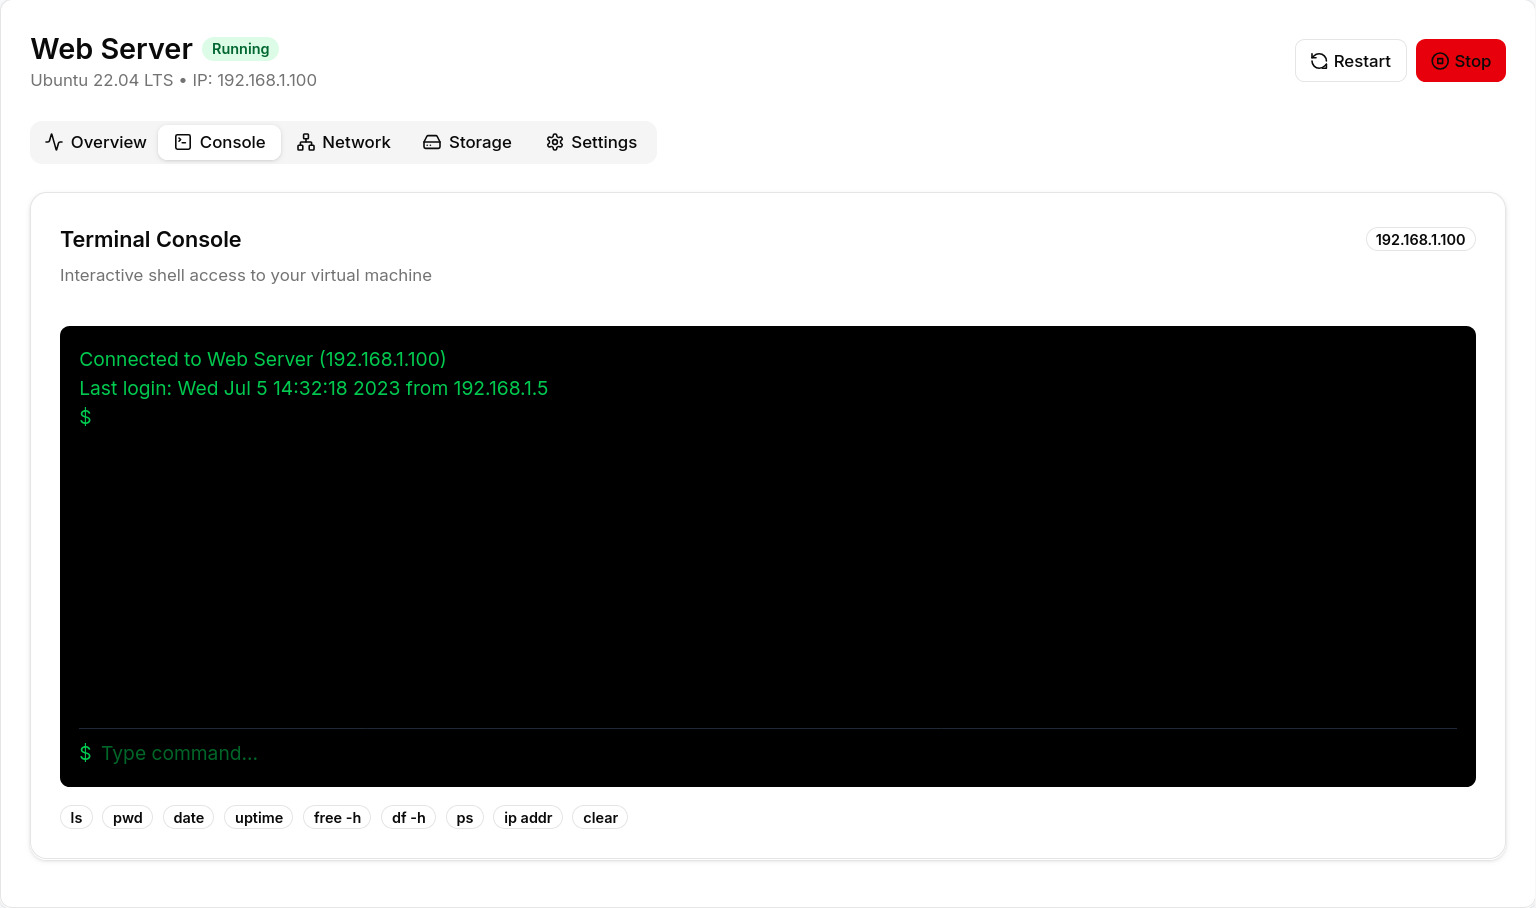
\includegraphics[width=0.85\textwidth]{it.jpeg} % Replace with your IT oriented practice image file
  \caption{Interface de pratique IT avec accès terminal à une machine virtuelle.}
  \label{fig:it_practice}
\end{figure}

\subsubsection{Interface de Pratique en Apprentissage Automatique (IA/ML)}
Un environnement dédié à l'apprentissage automatique a été créé. Il permet aux utilisateurs de :
\begin{itemize}
    \item Parcourir et sélectionner des jeux de données (datasets) depuis une bibliothèque intégrée ou en important les leurs (Voir Figure \ref{fig:ml_datasets}).
    \item Configurer et entraîner des modèles d'IA/ML simples directement sur la plateforme, avec des visualisations des étapes d'entraînement et des résultats (Voir Figure \ref{fig:ml_training}).
\end{itemize}
Cette interface vise à démystifier les concepts de l'IA et à offrir une première expérience pratique.


\begin{figure}[htbp]
  \centering
  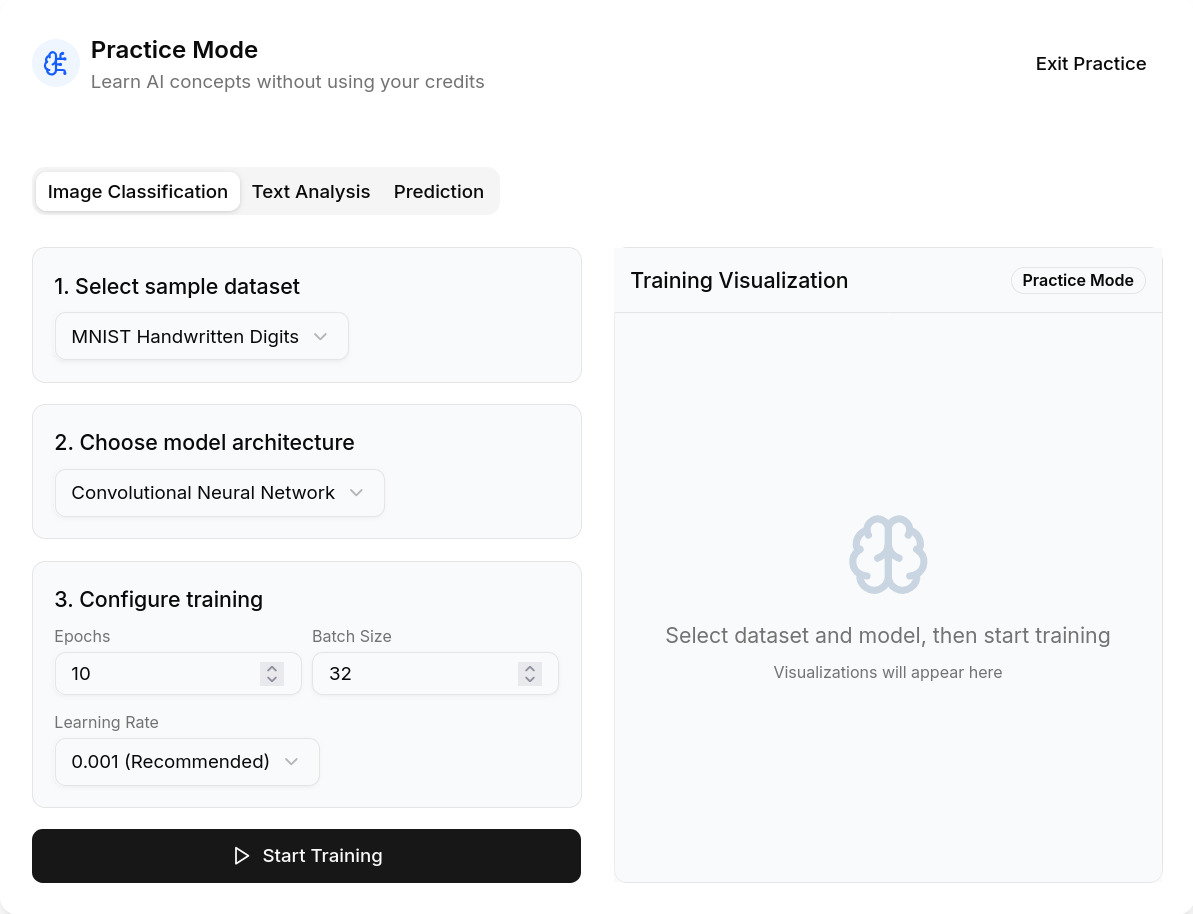
\includegraphics[width=0.85\textwidth]{ai_2.jpeg} % Replace with your ML model training image file
  \caption{Mode de pratique pour la configuration et l'entraînement de modèles d'IA/ML.}
  \label{fig:ml_training}
\end{figure}


\begin{figure}[htbp]
  \centering
  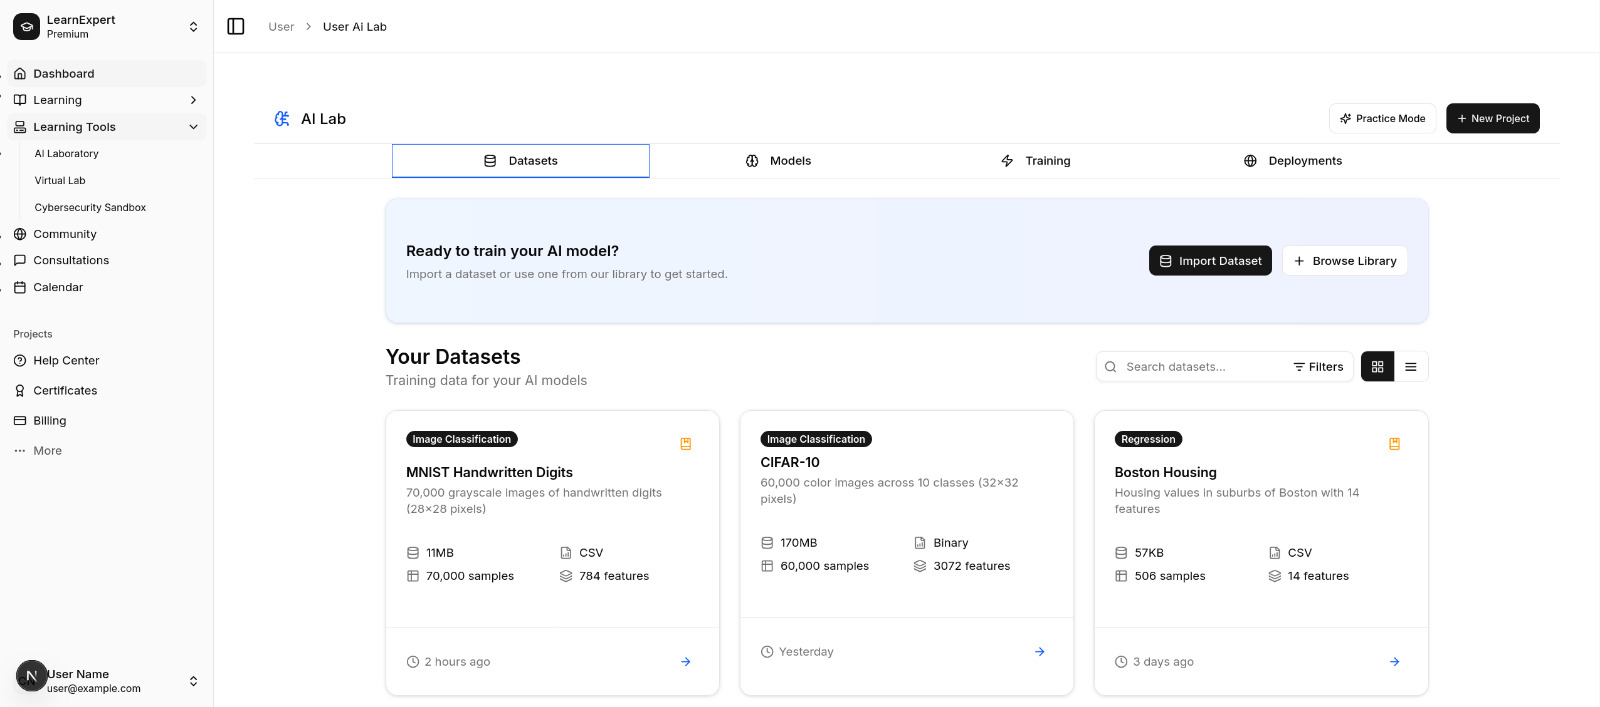
\includegraphics[width=0.85\textwidth]{ai_1.jpeg} % Replace with your ML dataset browsing image file
  \caption{Section de navigation et sélection des jeux de données pour la pratique IA/ML.}
  \label{fig:ml_datasets}
\end{figure}
\newpage

\subsection{Planification pour le Jour Suivant (Jeudi 29 Mai 2025)}

Pour la journée de demain, les activités prévues sont :
\begin{itemize}
  \item Commencer le développement des interfaces pour la section administrateur de la plateforme.
  \item Définir les fonctionnalités et l'architecture de l'interface de gestion des cours (côté administrateur/instructeur).
  \item Poursuivre la documentation technique des composants UI développés cette semaine.
\end{itemize}

\section{Conclusion}
La journée a été marquée par des avancées significatives dans l'enrichissement de l'offre premium de LearnExpert avec l'implémentation de quatre interfaces de pratique spécialisées. Ces modules pour l'algorithmique, la cybersécurité, les systèmes IT et l'IA/ML sont cruciaux pour offrir une valeur ajoutée concrète aux utilisateurs, en leur permettant de mettre en application les connaissances théoriques. L'accent mis sur l'interactivité et la simulation d'environnements réels vise à améliorer l'engagement et l'efficacité de l'apprentissage. Les travaux de demain se concentreront sur les aspects administratifs et de gestion de contenu de la plateforme.

\end{document}